\appendix
\addcontentsline{toc}{chapter}{Annexes}
\chapter*{Annexes}

\begin{figure}[ht]
    \centering
    \begin{subfigure}{0.37\textwidth}
        \includegraphics[width=\linewidth]{datas/state_of_the_art/opensfm_result_dino.png}
        \caption{}
    \end{subfigure}
    \begin{subfigure}{0.37\textwidth}
        \includegraphics[width=\linewidth]{datas/state_of_the_art/visualsfm_result_dino.png}
        \caption{}
    \end{subfigure}

    \begin{subfigure}{0.37\textwidth}
        \includegraphics[width=\linewidth]{datas/state_of_the_art/openmvg_openmvs_result_dino.png}
        \caption{}
    \end{subfigure}
    \begin{subfigure}{0.37\textwidth}
        \includegraphics[width=\linewidth]{datas/state_of_the_art/meshroom_result_dino.png}
        \caption{}
    \end{subfigure}

    \begin{subfigure}{0.37\textwidth}
        \includegraphics[width=\linewidth]{datas/state_of_the_art/regard3d_result_dino.png}
        \caption{}
    \end{subfigure}
    \begin{subfigure}{0.37\textwidth}
        \includegraphics[width=\linewidth]{datas/state_of_the_art/colmap_result_dino.png}
        \caption{}
    \end{subfigure}

    \caption{Résultats de l'état de l'art avec le dataset Dinosaure : (a)OpenSFM, (b)VisualSFM, (c)OpenMVG+OpenMVS, (d)Alicevision Meshroom, (e)Regard3D, (f)Colmap}
    \label{fig:results_etat_art}
\end{figure}

\begin{figure}[ht]
    \centering
    \begin{subfigure}{0.7\textwidth}
        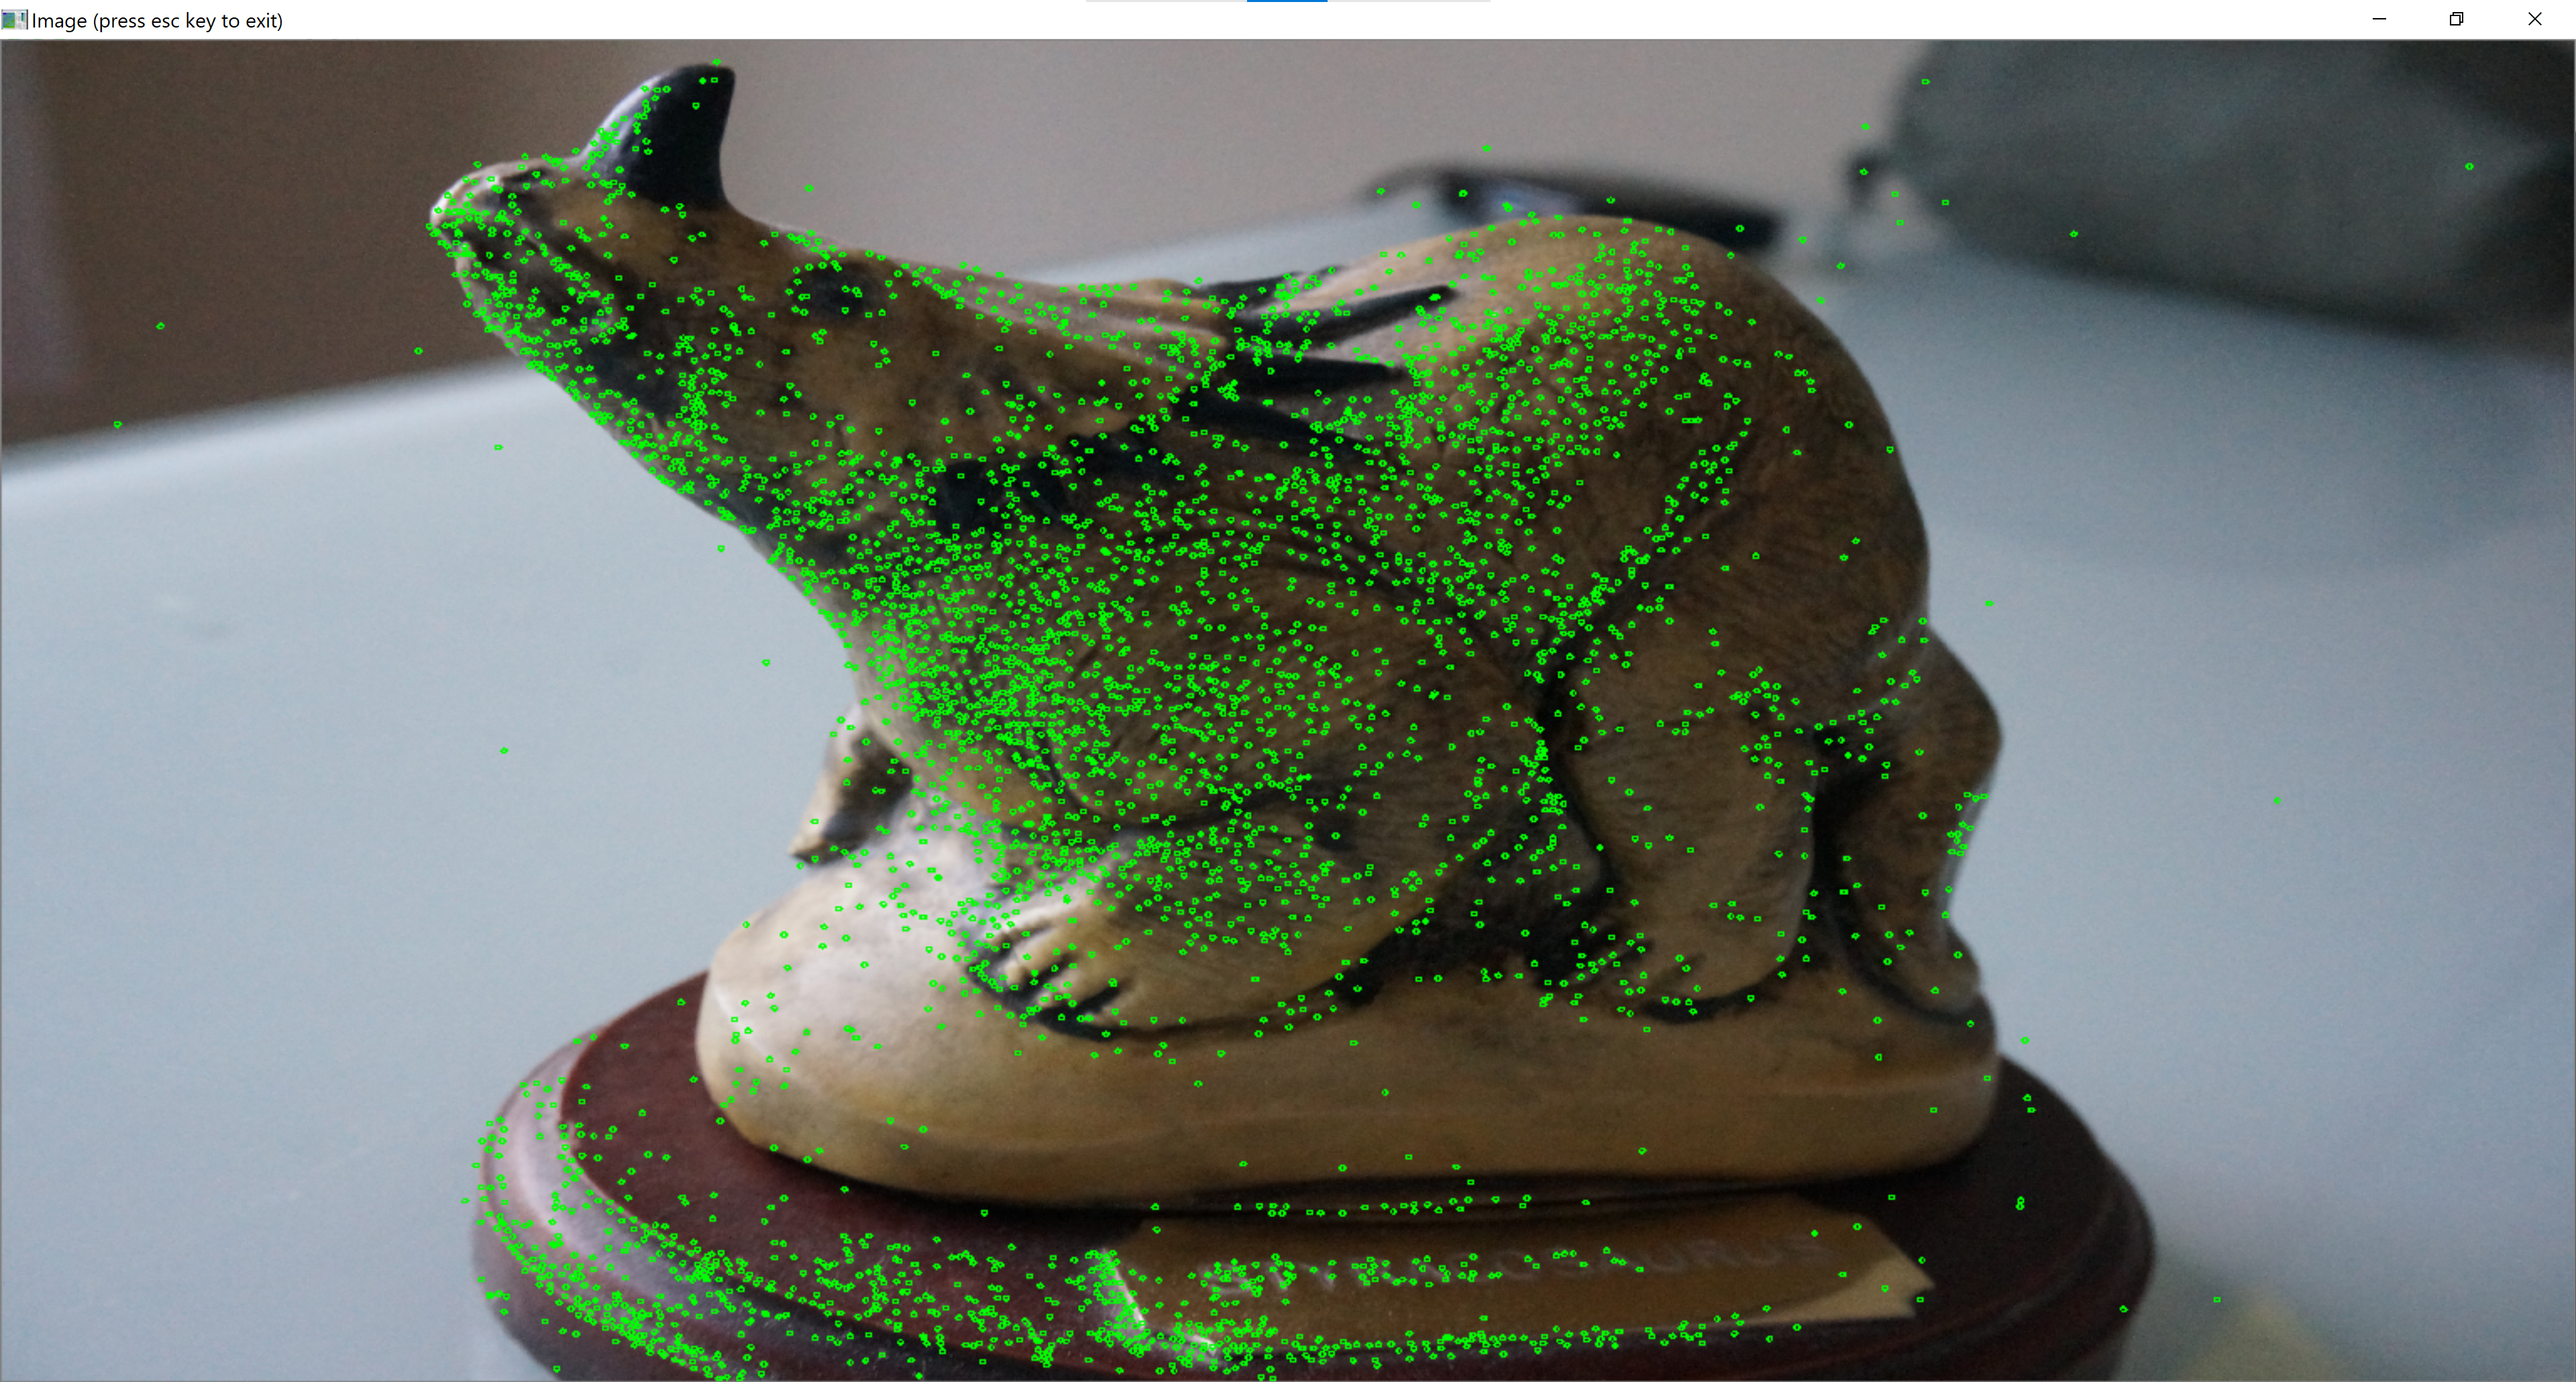
\includegraphics[width=\linewidth]{datas/helper/test_keyframe_dino.png}
    \end{subfigure}

    \begin{subfigure}{0.7\textwidth}
        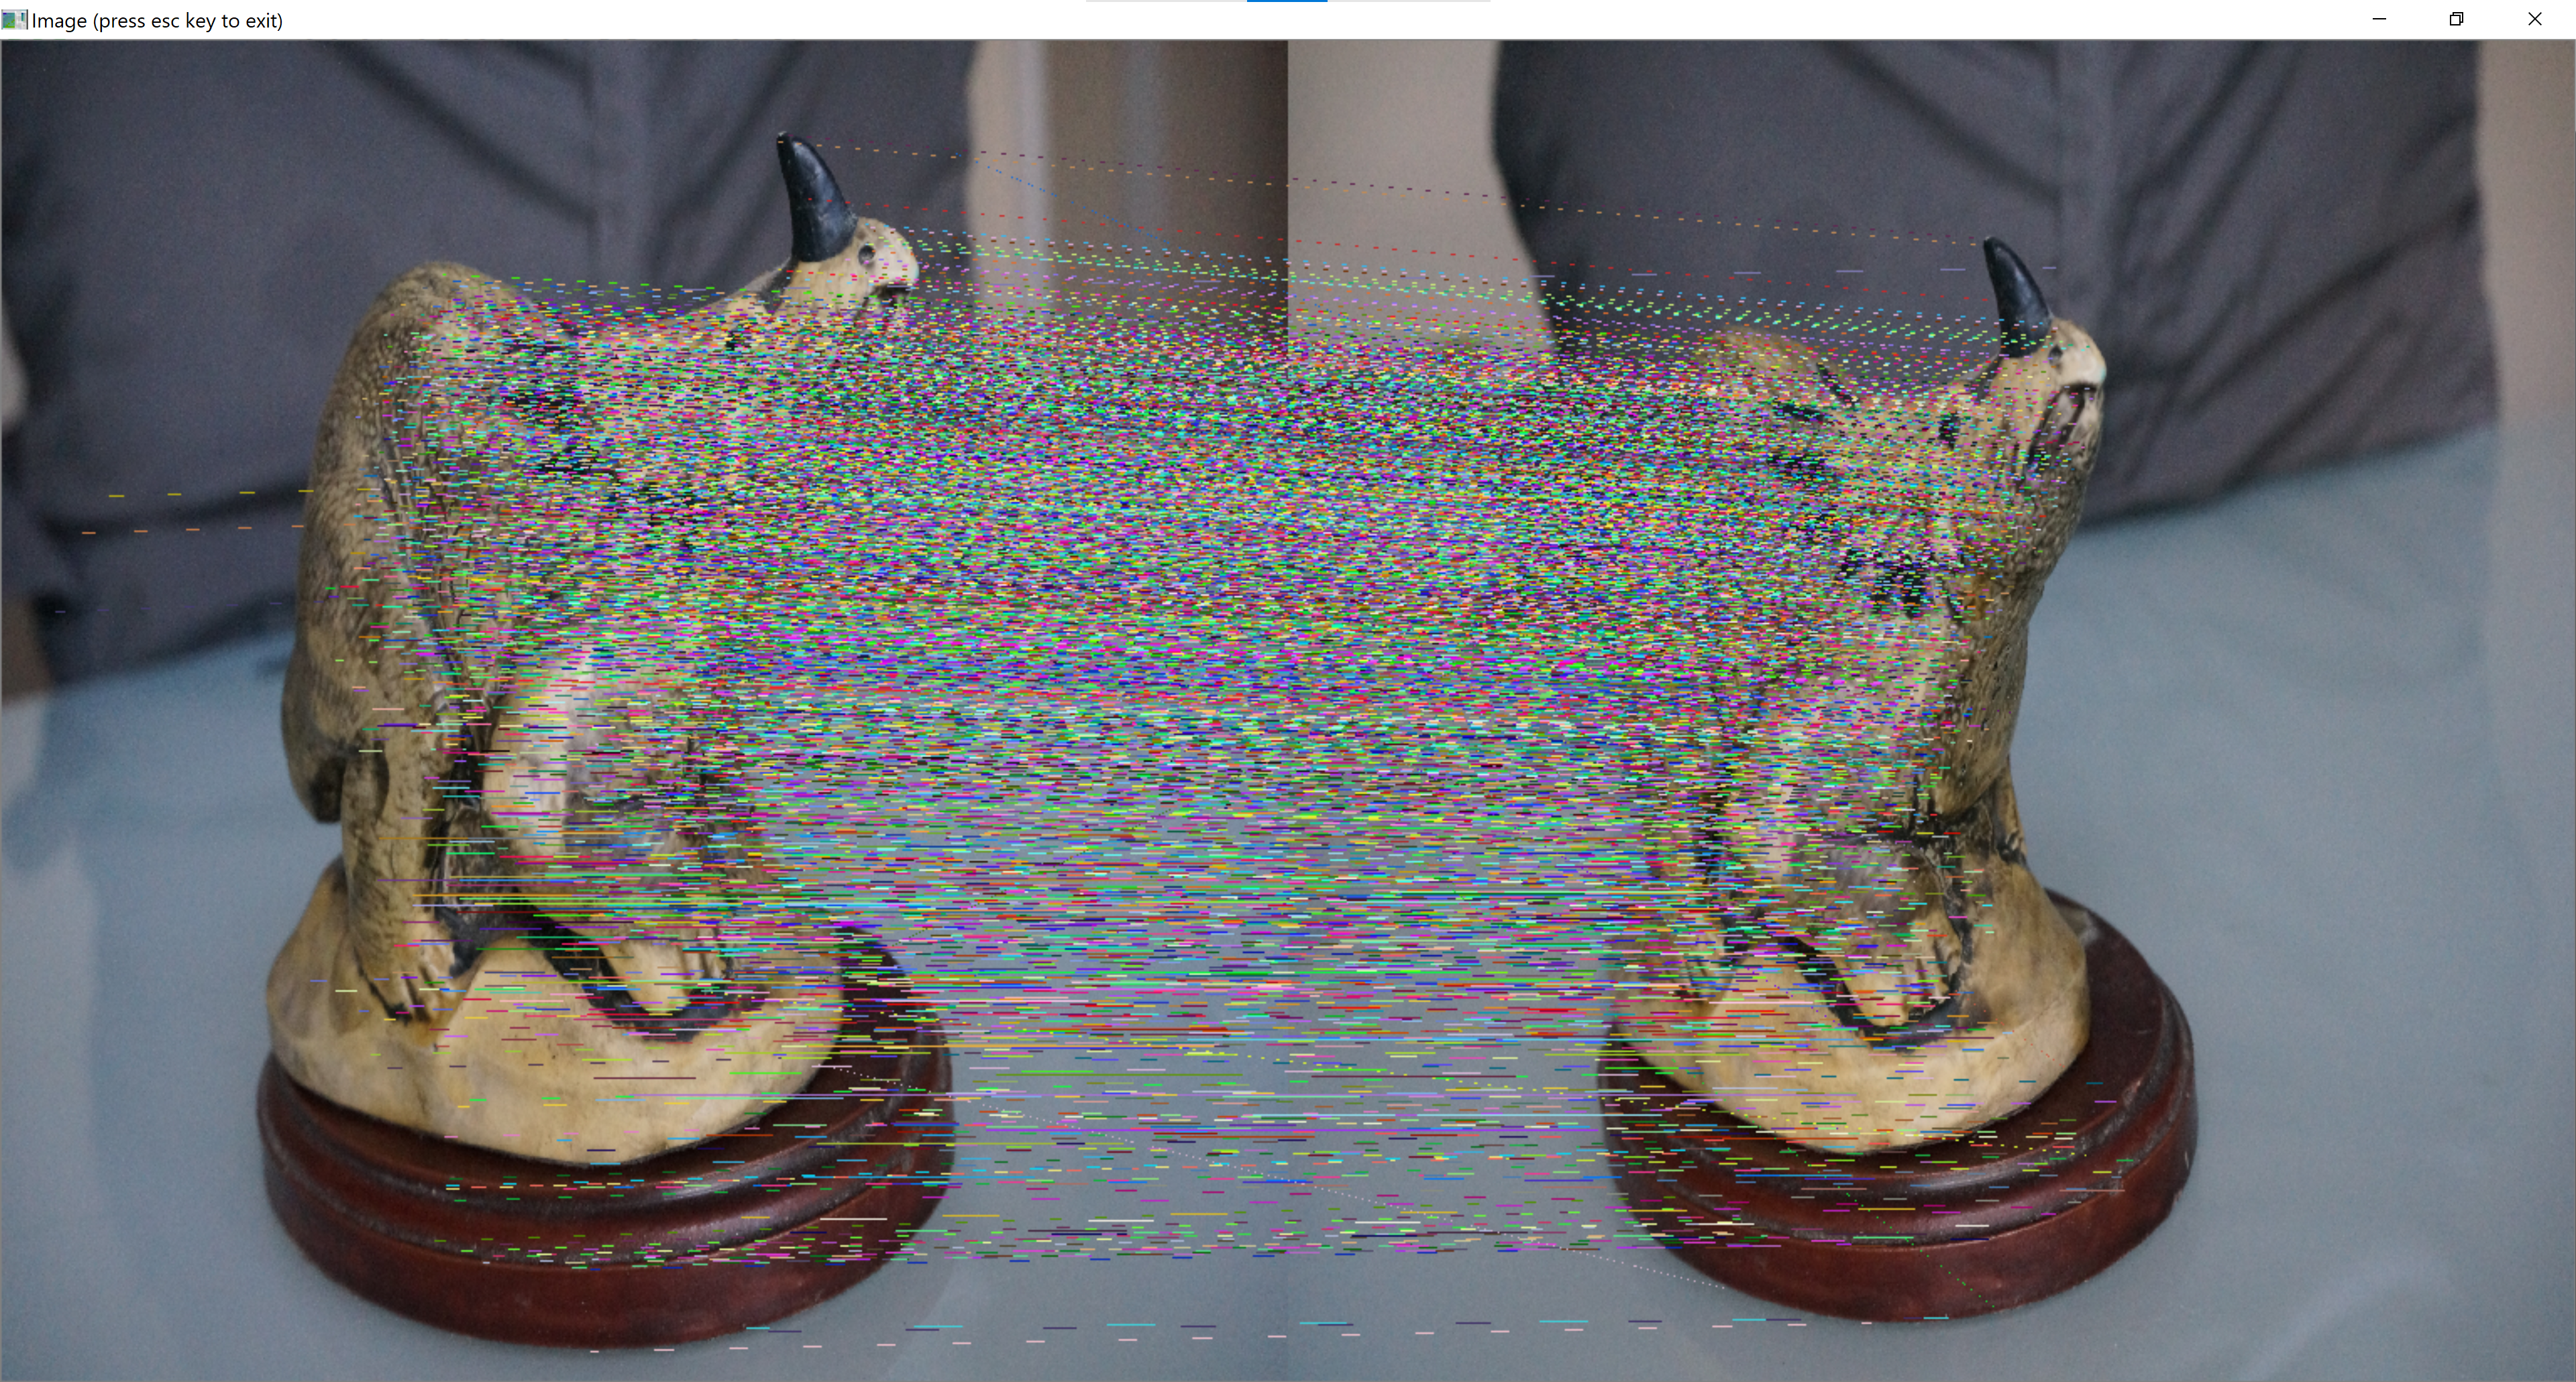
\includegraphics[width=\linewidth]{datas/helper/test_descriptors_dino.png}
    \end{subfigure}

    \begin{subfigure}{0.7\textwidth}
        \includegraphics[width=\linewidth]{datas/helper/test_pointcloud_dino.png}
    \end{subfigure}

    \caption{Résultats des tests pour le dataset Dinosaure}
    \label{fig:test_dino}
\end{figure}

\begin{figure}[ht]
    \centering
    \begin{subfigure}{0.7\textwidth}
        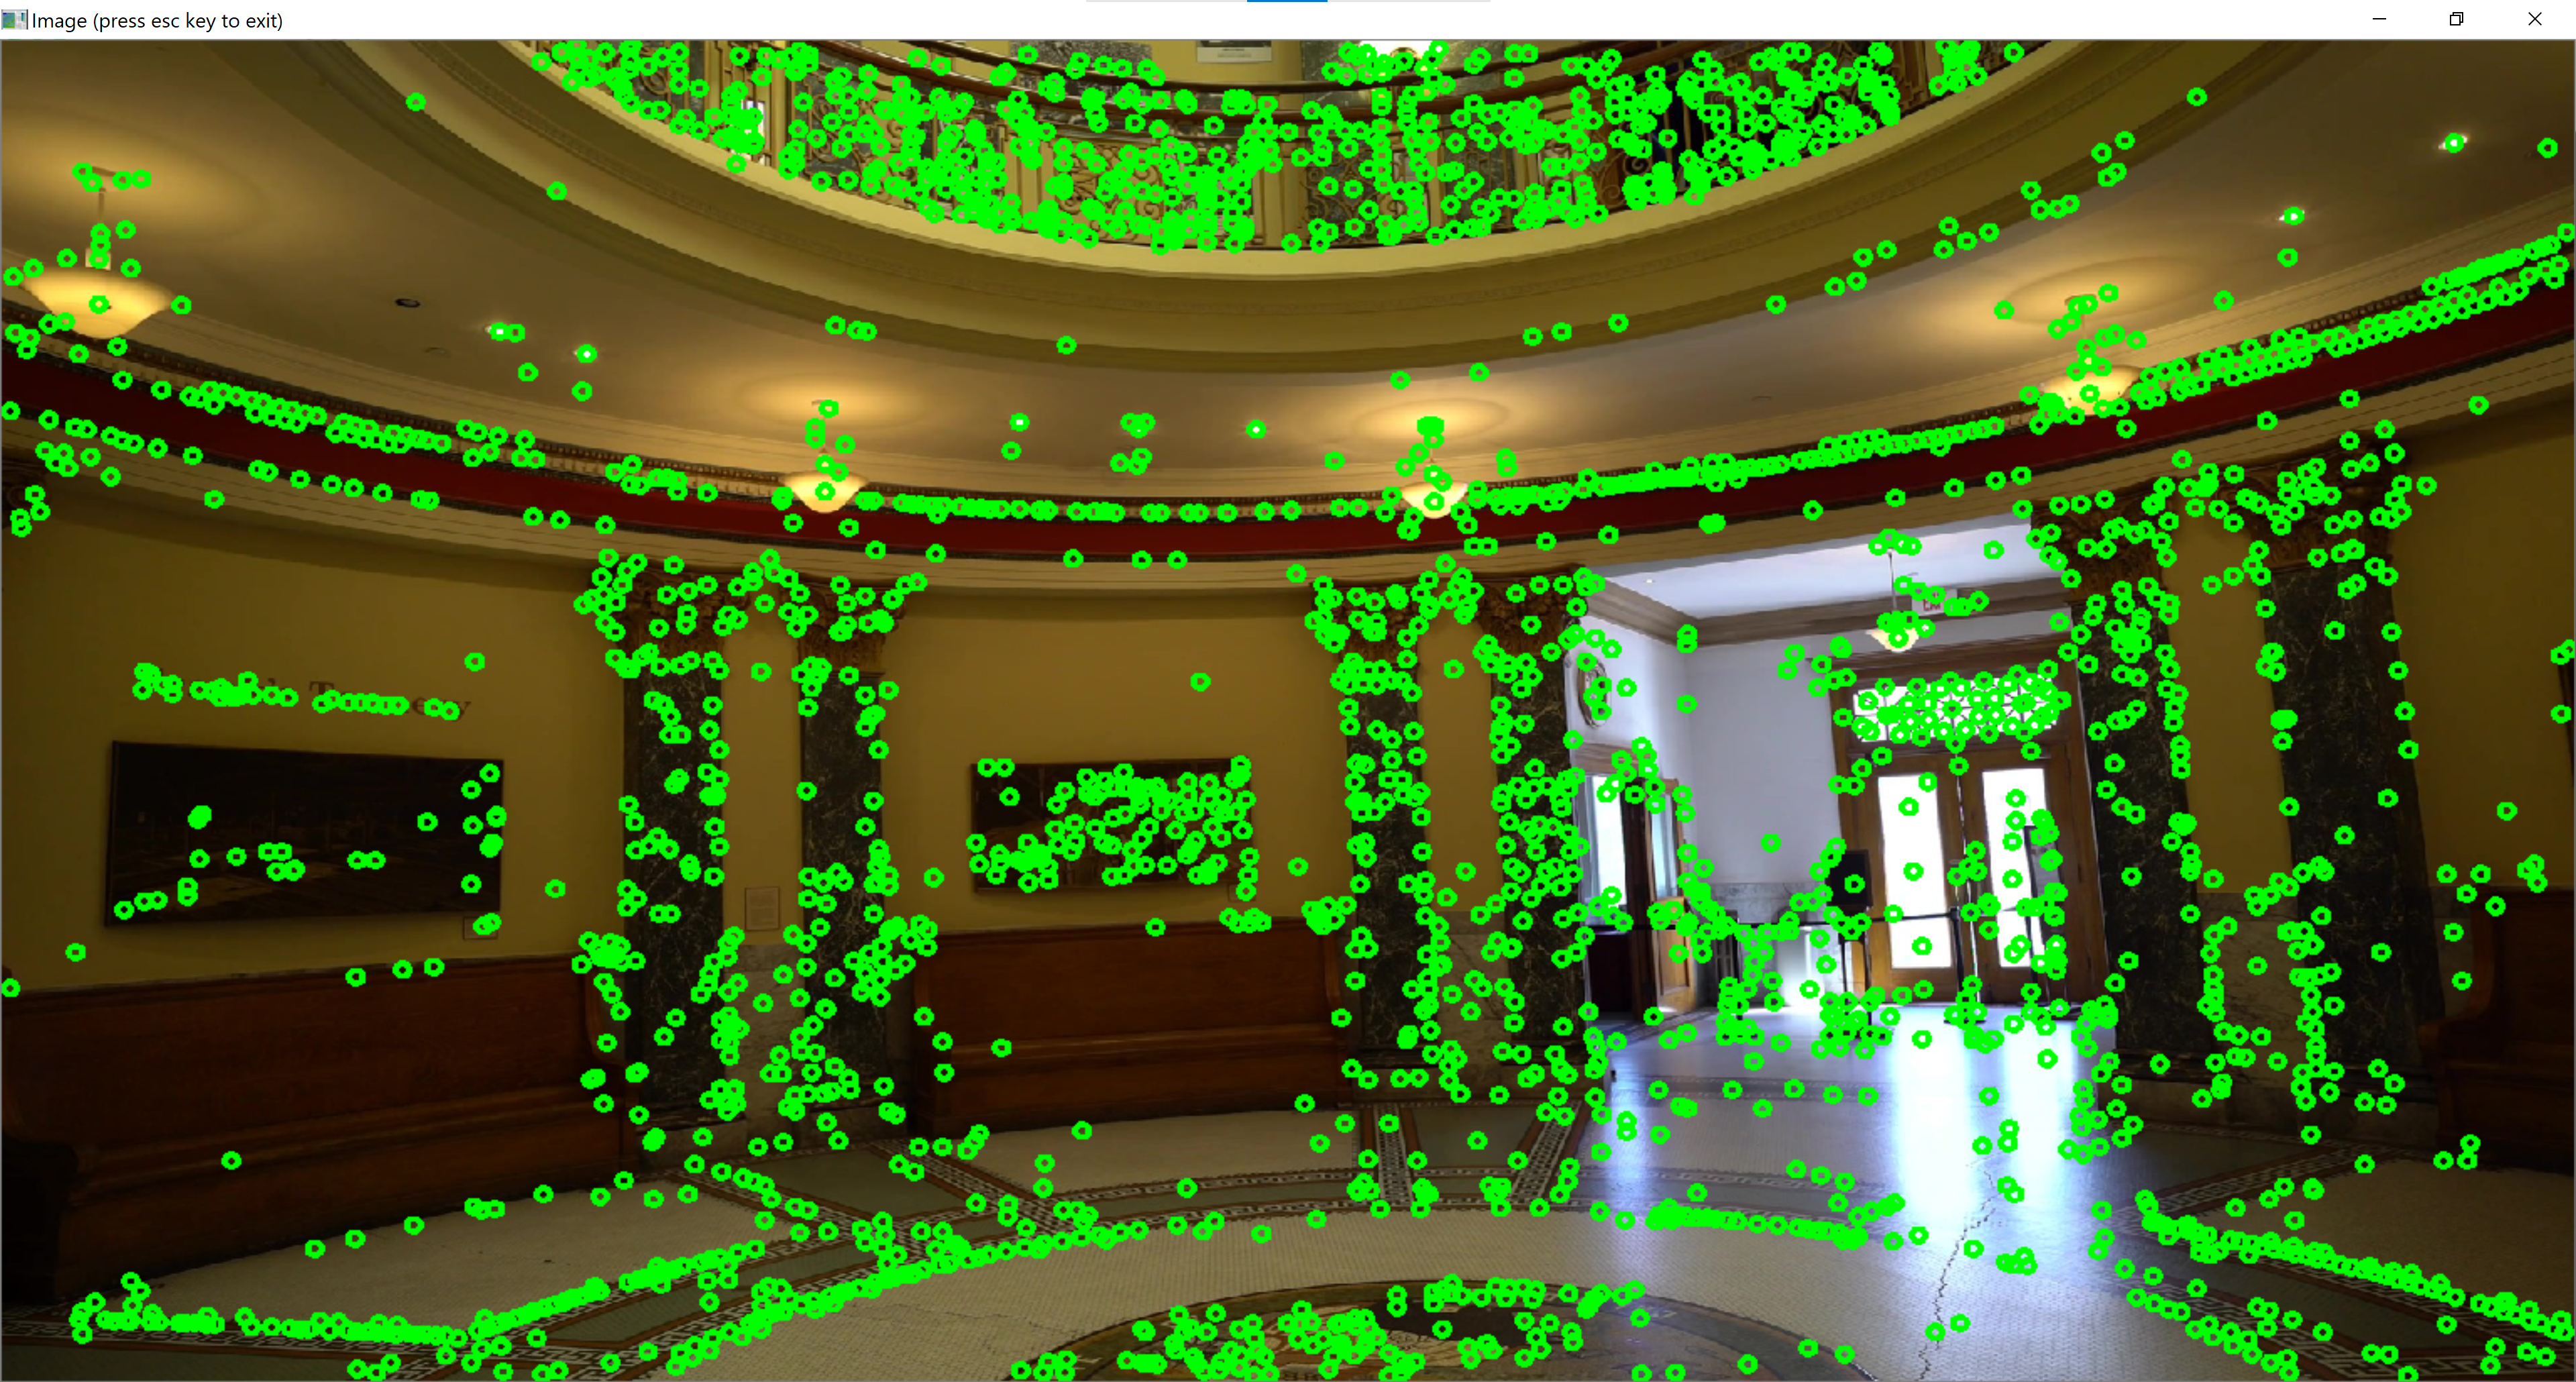
\includegraphics[width=\linewidth]{datas/helper/test_keyframe_museum.png}
    \end{subfigure}

    \begin{subfigure}{0.7\textwidth}
        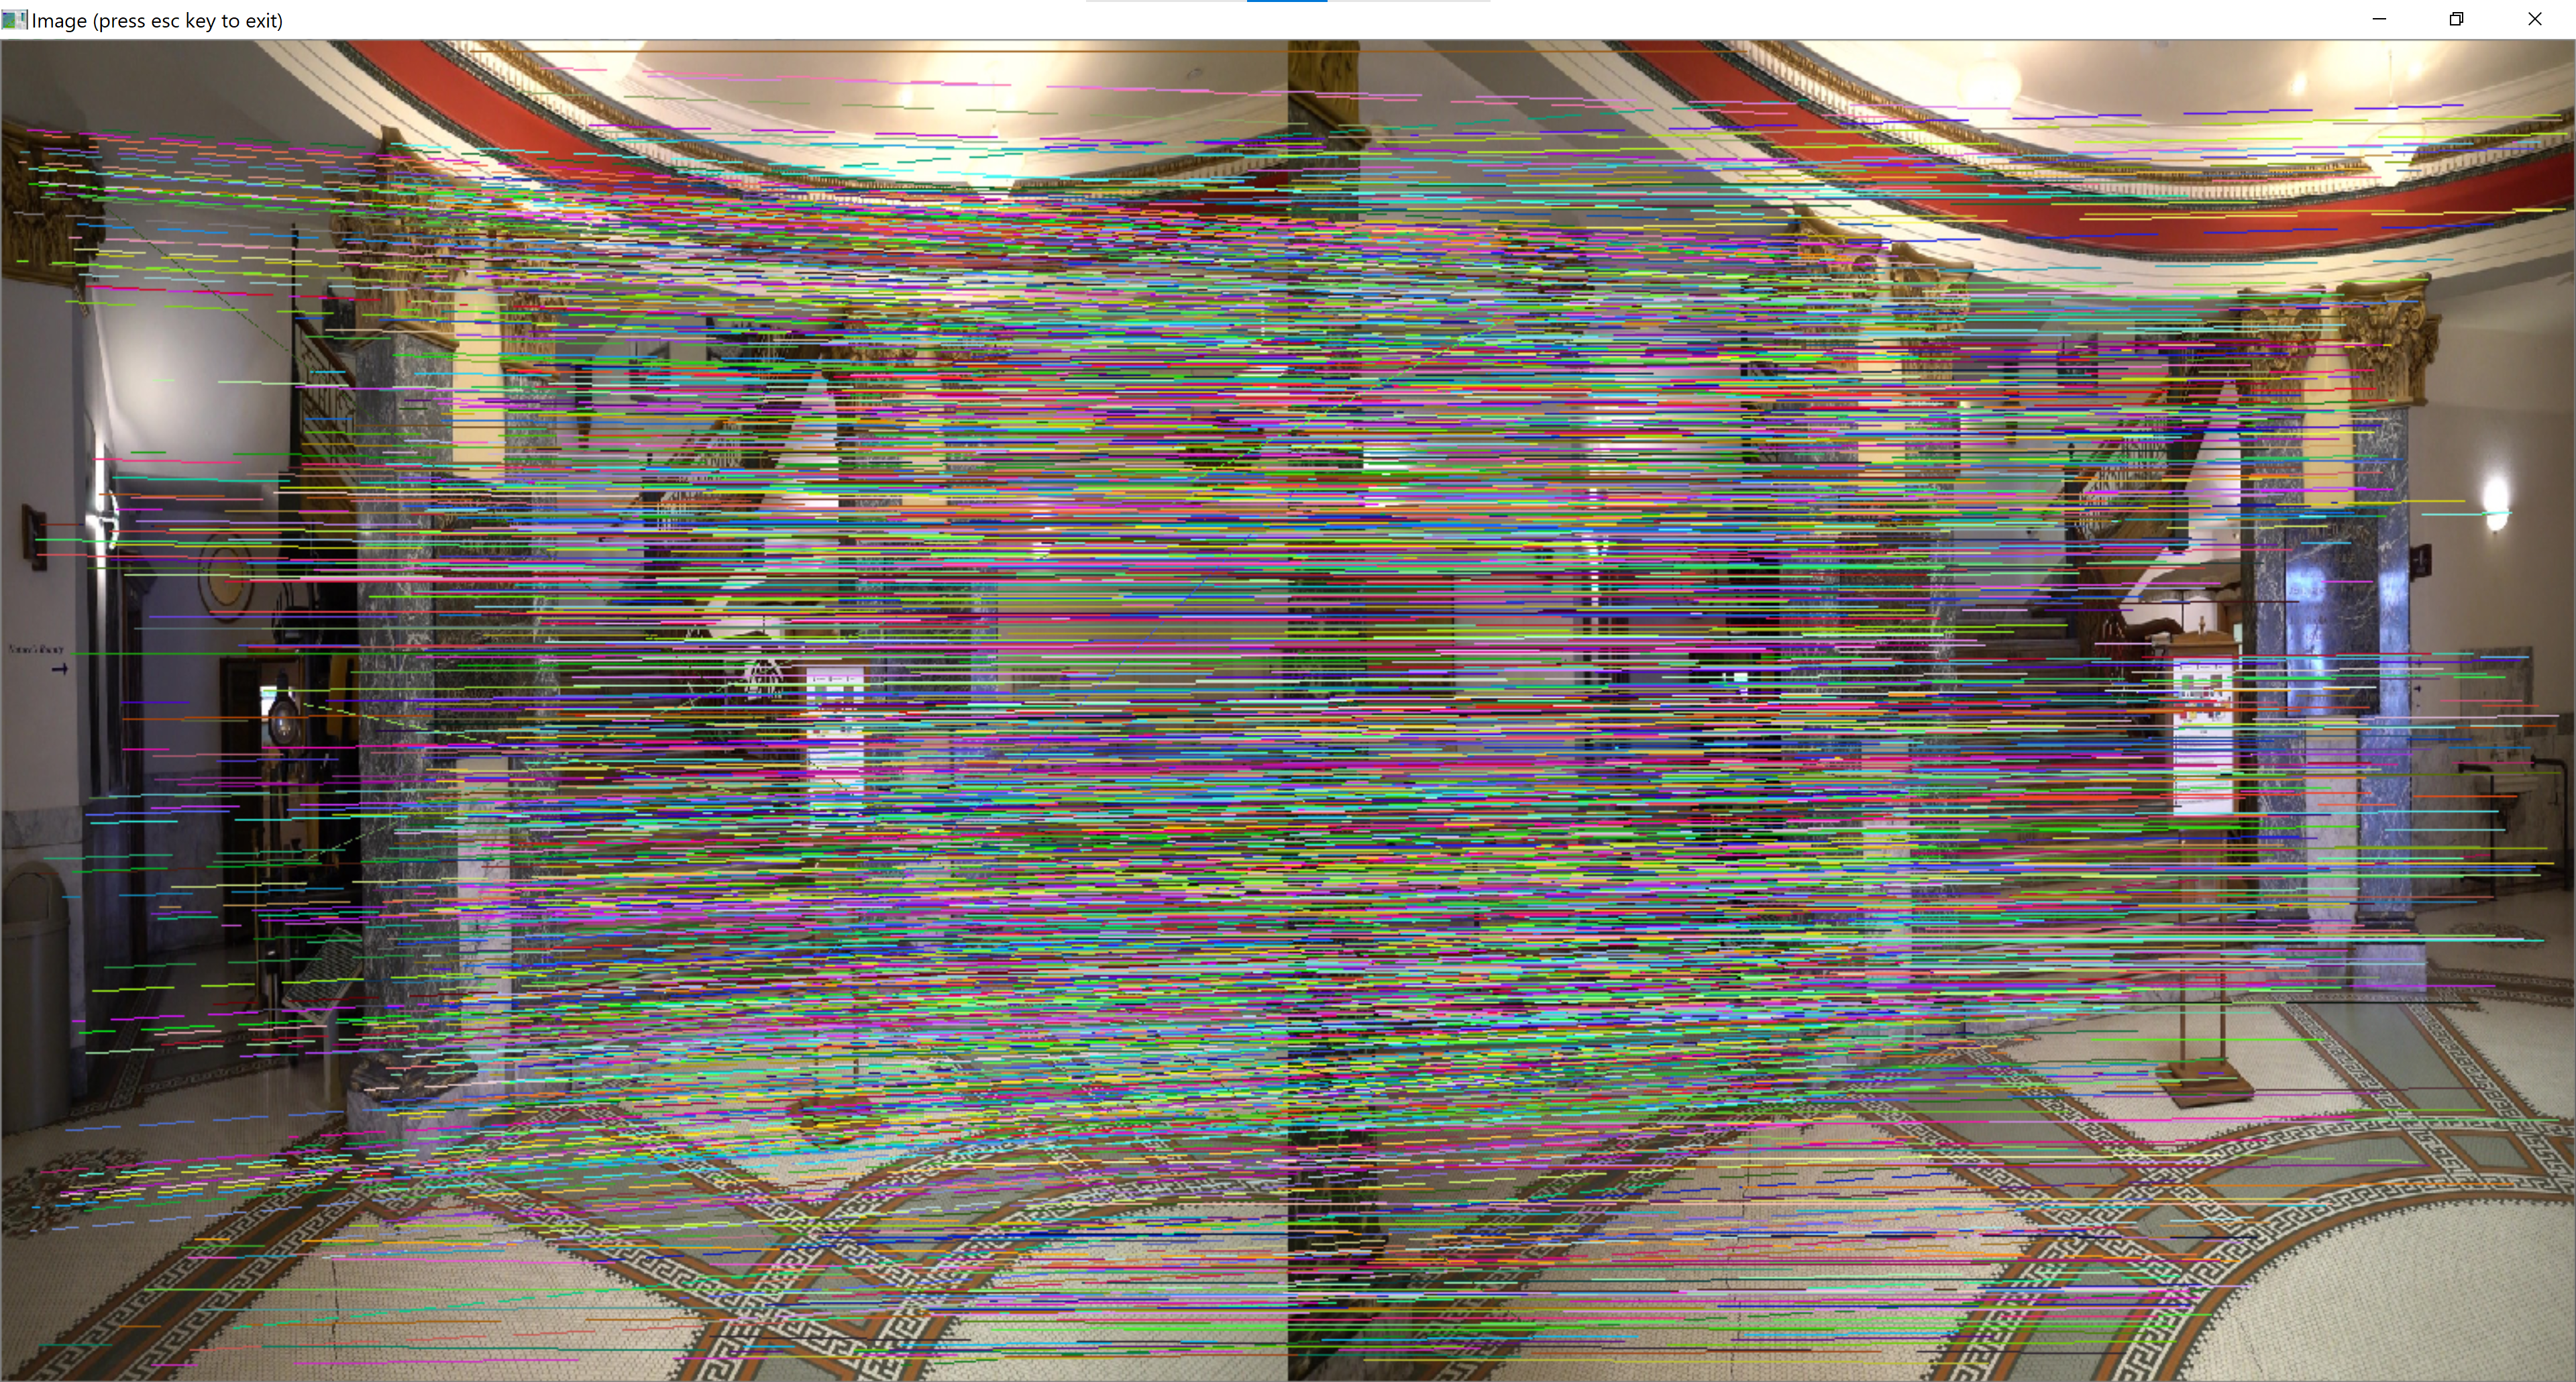
\includegraphics[width=\linewidth]{datas/helper/test_descriptors_museum.png}
    \end{subfigure}

    \begin{subfigure}{0.7\textwidth}
        \includegraphics[width=\linewidth]{datas/helper/test_pointcloud_museum.png}
    \end{subfigure}

    \caption{Résultats des tests pour le dataset Museum}
    \label{fig:test_museum}
\end{figure}